\documentclass[mathserif]{beamer}

\usepackage{microtype}
\usepackage{xparse}
\usepackage{amsmath}
\usepackage{amssymb}
\usepackage{mathtools}
\usepackage{graphicx}

\frenchspacing

\logo{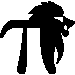
\includegraphics[width=0.07\textwidth]{../Logo}}

\usetheme{Rochester}
\usecolortheme{whale}

\setbeamertemplate{frametitle continuation}[from second][\hfill\insertcontinuationtext]

% Table of contents at start of each section
\AtBeginSection[] {%
	\begin{frame}
		\frametitle{Table of Contents}
		\tableofcontents[currentsection]
	\end{frame}
}

% Environments for math
\newenvironment{compactmath}[1][\normalsize]%
	{\begin{minipage}{\textwidth}\vspace{-0.5\baselineskip}#1\begin{equation*}}
	{\end{equation*}\end{minipage}}

\newenvironment{sizedmath}[1]%
	{\begingroup#1\begin{equation*}}
	{\end{equation*}\endgroup}

% Environments for consistent frame use
\newenvironment{namedframe}[1]%
	{\begin{frame}\frametitle{#1}\framesubtitle{\secname}}
	{\end{frame}}

\newenvironment{namedbreakframe}[1]%
	{\begin{frame}[allowframebreaks]\frametitle{#1}\framesubtitle{\secname}}
	{\end{frame}}

% Frames for emphasis
\newcommand{\sectionstart}[2]{\begin{frame}\frametitle{#1}\centering\Huge\secname\\\Large#2\end{frame}}
\newcommand{\bigframe}[1]{\begin{namedframe}{#1}\Huge\centering#1\end{namedframe}}

% Spacing commands
\newcommand{\sep}{\\\pause\vspace{1ex}}
\newcommand{\varsep}[1]{\\\pause\vspace{#1}}

\newcommand{\vertspace}{\\\vspace{1ex}}
\newcommand{\varvertspace}[1]{\\\vspace{#1}}

% Text formatting
\DeclareTextFontCommand{\emph}{\bfseries}

% Macros for math
\newcommand{\such}{\ |\ }
\DeclarePairedDelimiter{\ceil}{\lceil}{\rceil}
\DeclarePairedDelimiter{\floor}{\lfloor}{\rfloor}


\usepackage{amsthm}
\usepackage{array}

\setlength{\extrarowheight}{.1ex}

\title{Boolean Algebra}
\author{Vincent Macri}
\date{
\includegraphics{../LicenseLogo}\\\copyright{} Vincent Macri, 2017}

\newcommand{\xor}{\oplus}
\newcommand{\negate}[1]{\overline{#1}}

\begin{document}
	\frame{\titlepage}
	\section{Basics}
	\begin{namedframe}{What is boolean algebra}
		\begin{itemize}[<+->]
			\item A branch of mathematics dealing only with true and false values (usually called $1$ and $0$, respectively)
			\item Useful while considering logic
			\item Useful in computer science
		\end{itemize}
	\end{namedframe}
	\begin{namedframe}{Main operations}
		Boolean algebra has four important\footnote{There are other operations, but they are not as commonly used.} operations.
		\pause
		\begin{description}
			\item[$\neg A$] NOT (negation). Also written as $\negate{A}$.
			\item[$A \wedge B$] AND (conjunction). Also written as $A \cdot B$ or $AB$.
			\item[$A \xor B$] XOR (exclusive or).
			\item[$A \vee B$] OR (disjunction). Also written as $A + B$.
		\end{description}
		\pause
		Order of operations is \alert{BNAO}: brackets, NOT, AND, then OR.
		\pause
		\begin{alertblock}{Note on exclusive or's placement}
			\vspace{-0.5\baselineskip}
			There is no generally agreement on where to put XOR in the order of operations. It is commonly put between AND and OR (BNAXO), but you should always use brackets to avoid ambiguity.
		\end{alertblock}
	\end{namedframe}
	\section{Truth Tables}
	\begin{namedframe}{What is a truth table}
		A truth table is table of all possible input and output values of a boolean algebra statement.
		\pause

		They are similar to the multiplication tables you used in elementary school, but are much more powerful.
	\end{namedframe}
	\begin{namedframe}{Truth tables of main operations}
		\begin{center}
			\begin{minipage}[t]{0.45\textwidth}
				\pause
				\begin{table}
					\caption{AND}
					\begin{math}
						\begin{array}{|c|c|c|}
							\hline
							A & B & A \wedge B\\\hline
							0 & 0 & 0\\\hline
							0 & 1 & 0\\\hline
							1 & 0 & 0\\\hline
							1 & 1 & 1\\\hline
						\end{array}
					\end{math}
				\end{table}
				\varsep{-1.5\baselineskip}
				\begin{table}
					\caption{OR}
					\begin{math}
						\begin{array}{|c|c|c|}
							\hline
							A & B & A \vee B\\\hline
							0 & 0 & 0\\\hline
							0 & 1 & 1\\\hline
							1 & 0 & 1\\\hline
							1 & 1 & 1\\\hline
						\end{array}
					\end{math}
				\end{table}
			\end{minipage}
			\begin{minipage}[t]{0.45\textwidth}
				\pause
				\begin{table}
					\caption{XOR}
					\begin{math}
						\begin{array}{|c|c|c|}
							\hline
							A & B & A \xor B\\\hline
							0 & 0 & 0\\\hline
							0 & 1 & 1\\\hline
							1 & 0 & 1\\\hline
							1 & 1 & 0\\\hline
						\end{array}
					\end{math}
				\end{table}
				\varsep{-1.5\baselineskip}
				\begin{table}
					\caption{NOT}
					\begin{math}
						\begin{array}{|c|c|}
							\hline
							A & \neg A\\\hline
							0 & 1\\\hline
							1 & 0\\\hline
						\end{array}
					\end{math}
				\end{table}
			\end{minipage}
		\end{center}
	\end{namedframe}
	\section{Laws and Identities}
	\begin{namedframe}{Associativity, commutativity, and distributivity}
		Boolean algebra has many similar laws as regular algebra.

		For example, both $\wedge$ and $\vee$ follow the associative law and commutative laws, just like $\times$ and $+$.

		They also follow the distributive law.
		\begin{center}
			\pause
			\begin{minipage}{0.45\textwidth}
				\begin{block}{Associative law}
					\centering
					$A \cdot (B \cdot C) = (A \cdot B) \cdot C$

					$A + (B + C) = (A + B) + C$
				\end{block}
			\end{minipage}
			\pause
			\begin{minipage}{0.45\textwidth}
				\begin{block}{Commutative law}
					\centering
					$A \cdot B = B \cdot A$

					$A + B = B + A$
				\end{block}
			\end{minipage}
		\end{center}
		\pause
		\begin{block}{Distributive law}
			\centering
			$A \cdot (B + C) = AB + AC$
		\end{block}
	\end{namedframe}
	\begin{namedframe}{Identities}
		Some of the identities in boolean algebra are the same as in regular algebra.
		\begin{itemize}[<+(1)->]
			\item $A + 0 = A$
			\item $A \cdot 1 = A$
			\item $A \cdot 0 = 0$
		\end{itemize}
		\pause
		However, some of the identities which are true in boolean algebra do not work in regular algebra.
		\begin{center}
			\begin{minipage}{0.25\textwidth}
				\begin{itemize}[<+(1)->]
					\item $A + 1 = 1$
					\item $A + A = A$
					\item $A \cdot A = A$
				\end{itemize}
			\end{minipage}
			\begin{minipage}{0.65\textwidth}
				\begin{itemize}[<+(1)->]
					\item $A \cdot (A + B) = A$
					\item $A + AB = A$
					\item $A + BC = (A + B) \cdot (A + C)$
				\end{itemize}
			\end{minipage}
		\end{center}
	\end{namedframe}
	\begin{namedframe}{Identities with NOT}
		These are some identities involving NOT:
		\pause
		\[\negate{\negate{A}} = A\]
		\pause
		\[\negate{A} + A = 1\]
		\pause
		\[\negate{A} \cdot A = 0\]
	\end{namedframe}
	\begin{namedframe}{De Morgan's laws}
		Another set of identities useful in boolean algebra are De Morgan's laws.
		\begin{center}
			\pause
			\begin{minipage}{0.425\textwidth}
				\centering
				\begin{block}{NOT OR}
					\begin{compactmath}
						\negate{A + B} = \negate{A} \cdot \negate{B}
					\end{compactmath}
				\end{block}
				\begin{math}
					\begin{array}{|c|c|c|c|}
						\hline
						A & B & \negate{A + B} & \negate{A} \cdot \negate{B}\\\hline
						0 & 0 &  1             &  1                         \\\hline
						0 & 1 &  0             &  0                         \\\hline
						1 & 0 &  0             &  0                         \\\hline
						1 & 1 &  0             &  0                         \\\hline
					\end{array}
				\end{math}
			\end{minipage}
			\hspace{0.025\textwidth}
			\pause
			\begin{minipage}{0.425\textwidth}
				\centering
				\begin{block}{NOT AND}
					\begin{compactmath}
						\negate{A \cdot B} = \negate{A} + \negate{B}
					\end{compactmath}
				\end{block}
				\begin{math}
					\begin{array}{|c|c|c|c|}
						\hline
						A & B & \negate{A \cdot B} & \negate{A} + \negate{B}\\\hline
						0 & 0 &  1             &  1                         \\\hline
						0 & 1 &  1             &  1                         \\\hline
						1 & 0 &  1             &  1                         \\\hline
						1 & 1 &  0             &  0                         \\\hline
					\end{array}
				\end{math}
			\end{minipage}
		\end{center}
	\end{namedframe}
	\section{Practice}
	\begin{namedframe}{Simplify}
		\begin{compactmath}[\Large]
			A + AB \cdot B + C \cdot \negate{C}
		\end{compactmath}
		\pause
		\begin{align*}
			\uncover<+->{&\phantom{{}={}}A + (AB \cdot B) + (C \cdot \negate{C})\\}
			\uncover<+->{&=A + (AB) + (0)\\}
			\uncover<+->{&=A + AB\\}
			\uncover<+->{&=A}
		\end{align*}
		\uncover<+->{$\therefore A + AB \cdot B + C \cdot \negate{C} = A$}
	\end{namedframe}
\end{document}
